\qquad O Selection Sort é um algoritmo de ordenação por comparação baseado
na ideia de, repetidamente, selecionar o menor elemento ainda não
ordenado e colocá-lo em sua posição final. É um dos algoritmos mais
intuitivos: em vez de inserir elementos em uma sequência já ordenada
(como faz o Insertion Sort), o Selection Sort constrói a parte
ordenada do vetor da esquerda para a direita, sempre buscando, entre
os elementos restantes, aquele que deve ocupar a próxima posição.

\qquad O algoritmo percorre o vetor com um índice \textit{i}, de 0 até
tamanho-2. Para cada posição \textit{i}, é feita uma busca linear pelo
menor elemento entre as posições \textit{i} e tamanho-1. Encontrado o
menor elemento, ele é trocado de lugar com o elemento da posição
\textit{i} (a troca só é realizada se o menor encontrado não estiver
já na posição \textit{i}). Repetindo esse processo para todas as
posições, o vetor fica completamente ordenado em ordem crescente ao
final da execução.

\qquad A seguir apresenta-se a implementação utilizada neste trabalho, em
C++, correspondente à função \texttt{SelectionSort\_versao1}:

\begin{verbatim}
void SelectionSort_versao1(int *vetor, int tamanho) {
    int menor, aux;
    for (int i = 0; i < tamanho - 1; i++) {
        menor = i;
        for (int j = i + 1; j < tamanho; j++) {
            if (vetor[j] < vetor[menor]) {
                menor = j;
            }
        }
        if (menor != i) {
            aux = vetor[i];
            vetor[i] = vetor[menor];
            vetor[menor] = aux;
        }
    }
}
\end{verbatim}

\qquad Uma característica marcante do Selection Sort, explorada em detalhes
na análise de complexidade deste capítulo, é que o número de
\textit{comparações} realizadas não depende de a entrada já estar
ordenada, invertida ou embaralhada: a busca pelo menor elemento
sempre percorre integralmente os elementos restantes. Isso o
diferencia do Insertion Sort e do Bubble Sort, que se beneficiam de
entradas parcialmente ordenadas. A única grandeza que varia com o
tipo de entrada é o número de \textit{trocas}, que é, no máximo,
tamanho-1 em qualquer caso — uma quantidade desprezível diante do
número de comparações.

\subsection{Teste de Mesa Manual}

\qquad Nesta seção deve ser inserida a digitalização do teste de mesa
manual do Selection Sort, realizado à mão com um exemplo de entrada
diferente dos exemplos trabalhados em sala de aula, conforme exigido
pelo enunciado do trabalho. Substitua a imagem de exemplo abaixo pela
digitalização (foto ou escaneamento) do teste de mesa manuscrito.

\begin{figure}[htbp]
    \centering
    % Substitua o arquivo abaixo pela digitalizacao do teste de mesa manuscrito
    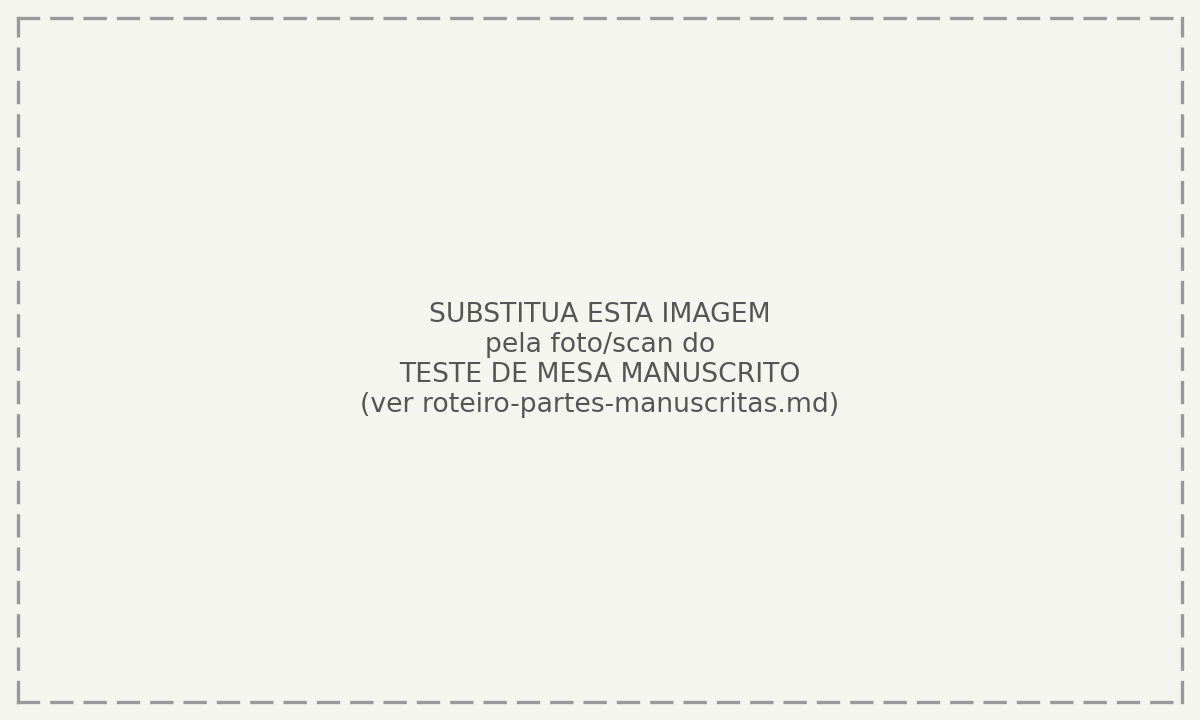
\includegraphics[width=14cm]{Imagens/Selection Sort/teste_de_mesa.png}
    \caption{Teste de mesa manual do algoritmo Selection Sort}
    \label{fig:teste_mesa_selection}
\end{figure}
